% Options for packages loaded elsewhere
\PassOptionsToPackage{unicode}{hyperref}
\PassOptionsToPackage{hyphens}{url}
%
\documentclass[
]{article}
\usepackage{amsmath,amssymb}
\usepackage{iftex}
\ifPDFTeX
  \usepackage[T1]{fontenc}
  \usepackage[utf8]{inputenc}
  \usepackage{textcomp} % provide euro and other symbols
\else % if luatex or xetex
  \usepackage{unicode-math} % this also loads fontspec
  \defaultfontfeatures{Scale=MatchLowercase}
  \defaultfontfeatures[\rmfamily]{Ligatures=TeX,Scale=1}
\fi
\usepackage{lmodern}
\ifPDFTeX\else
  % xetex/luatex font selection
\fi
% Use upquote if available, for straight quotes in verbatim environments
\IfFileExists{upquote.sty}{\usepackage{upquote}}{}
\IfFileExists{microtype.sty}{% use microtype if available
  \usepackage[]{microtype}
  \UseMicrotypeSet[protrusion]{basicmath} % disable protrusion for tt fonts
}{}
\makeatletter
\@ifundefined{KOMAClassName}{% if non-KOMA class
  \IfFileExists{parskip.sty}{%
    \usepackage{parskip}
  }{% else
    \setlength{\parindent}{0pt}
    \setlength{\parskip}{6pt plus 2pt minus 1pt}}
}{% if KOMA class
  \KOMAoptions{parskip=half}}
\makeatother
\usepackage{xcolor}
\usepackage[margin=1in]{geometry}
\usepackage{color}
\usepackage{fancyvrb}
\newcommand{\VerbBar}{|}
\newcommand{\VERB}{\Verb[commandchars=\\\{\}]}
\DefineVerbatimEnvironment{Highlighting}{Verbatim}{commandchars=\\\{\}}
% Add ',fontsize=\small' for more characters per line
\usepackage{framed}
\definecolor{shadecolor}{RGB}{248,248,248}
\newenvironment{Shaded}{\begin{snugshade}}{\end{snugshade}}
\newcommand{\AlertTok}[1]{\textcolor[rgb]{0.94,0.16,0.16}{#1}}
\newcommand{\AnnotationTok}[1]{\textcolor[rgb]{0.56,0.35,0.01}{\textbf{\textit{#1}}}}
\newcommand{\AttributeTok}[1]{\textcolor[rgb]{0.13,0.29,0.53}{#1}}
\newcommand{\BaseNTok}[1]{\textcolor[rgb]{0.00,0.00,0.81}{#1}}
\newcommand{\BuiltInTok}[1]{#1}
\newcommand{\CharTok}[1]{\textcolor[rgb]{0.31,0.60,0.02}{#1}}
\newcommand{\CommentTok}[1]{\textcolor[rgb]{0.56,0.35,0.01}{\textit{#1}}}
\newcommand{\CommentVarTok}[1]{\textcolor[rgb]{0.56,0.35,0.01}{\textbf{\textit{#1}}}}
\newcommand{\ConstantTok}[1]{\textcolor[rgb]{0.56,0.35,0.01}{#1}}
\newcommand{\ControlFlowTok}[1]{\textcolor[rgb]{0.13,0.29,0.53}{\textbf{#1}}}
\newcommand{\DataTypeTok}[1]{\textcolor[rgb]{0.13,0.29,0.53}{#1}}
\newcommand{\DecValTok}[1]{\textcolor[rgb]{0.00,0.00,0.81}{#1}}
\newcommand{\DocumentationTok}[1]{\textcolor[rgb]{0.56,0.35,0.01}{\textbf{\textit{#1}}}}
\newcommand{\ErrorTok}[1]{\textcolor[rgb]{0.64,0.00,0.00}{\textbf{#1}}}
\newcommand{\ExtensionTok}[1]{#1}
\newcommand{\FloatTok}[1]{\textcolor[rgb]{0.00,0.00,0.81}{#1}}
\newcommand{\FunctionTok}[1]{\textcolor[rgb]{0.13,0.29,0.53}{\textbf{#1}}}
\newcommand{\ImportTok}[1]{#1}
\newcommand{\InformationTok}[1]{\textcolor[rgb]{0.56,0.35,0.01}{\textbf{\textit{#1}}}}
\newcommand{\KeywordTok}[1]{\textcolor[rgb]{0.13,0.29,0.53}{\textbf{#1}}}
\newcommand{\NormalTok}[1]{#1}
\newcommand{\OperatorTok}[1]{\textcolor[rgb]{0.81,0.36,0.00}{\textbf{#1}}}
\newcommand{\OtherTok}[1]{\textcolor[rgb]{0.56,0.35,0.01}{#1}}
\newcommand{\PreprocessorTok}[1]{\textcolor[rgb]{0.56,0.35,0.01}{\textit{#1}}}
\newcommand{\RegionMarkerTok}[1]{#1}
\newcommand{\SpecialCharTok}[1]{\textcolor[rgb]{0.81,0.36,0.00}{\textbf{#1}}}
\newcommand{\SpecialStringTok}[1]{\textcolor[rgb]{0.31,0.60,0.02}{#1}}
\newcommand{\StringTok}[1]{\textcolor[rgb]{0.31,0.60,0.02}{#1}}
\newcommand{\VariableTok}[1]{\textcolor[rgb]{0.00,0.00,0.00}{#1}}
\newcommand{\VerbatimStringTok}[1]{\textcolor[rgb]{0.31,0.60,0.02}{#1}}
\newcommand{\WarningTok}[1]{\textcolor[rgb]{0.56,0.35,0.01}{\textbf{\textit{#1}}}}
\usepackage{longtable,booktabs,array}
\usepackage{calc} % for calculating minipage widths
% Correct order of tables after \paragraph or \subparagraph
\usepackage{etoolbox}
\makeatletter
\patchcmd\longtable{\par}{\if@noskipsec\mbox{}\fi\par}{}{}
\makeatother
% Allow footnotes in longtable head/foot
\IfFileExists{footnotehyper.sty}{\usepackage{footnotehyper}}{\usepackage{footnote}}
\makesavenoteenv{longtable}
\usepackage{graphicx}
\makeatletter
\def\maxwidth{\ifdim\Gin@nat@width>\linewidth\linewidth\else\Gin@nat@width\fi}
\def\maxheight{\ifdim\Gin@nat@height>\textheight\textheight\else\Gin@nat@height\fi}
\makeatother
% Scale images if necessary, so that they will not overflow the page
% margins by default, and it is still possible to overwrite the defaults
% using explicit options in \includegraphics[width, height, ...]{}
\setkeys{Gin}{width=\maxwidth,height=\maxheight,keepaspectratio}
% Set default figure placement to htbp
\makeatletter
\def\fps@figure{htbp}
\makeatother
\setlength{\emergencystretch}{3em} % prevent overfull lines
\providecommand{\tightlist}{%
  \setlength{\itemsep}{0pt}\setlength{\parskip}{0pt}}
\setcounter{secnumdepth}{-\maxdimen} % remove section numbering
\ifLuaTeX
  \usepackage{selnolig}  % disable illegal ligatures
\fi
\IfFileExists{bookmark.sty}{\usepackage{bookmark}}{\usepackage{hyperref}}
\IfFileExists{xurl.sty}{\usepackage{xurl}}{} % add URL line breaks if available
\urlstyle{same}
\hypersetup{
  pdftitle={Documento de cambios},
  pdfauthor={Ángela Alarcón Ballester, Lucía Ponce Salmerón y Carlos Sánchez Polo},
  hidelinks,
  pdfcreator={LaTeX via pandoc}}

\title{Documento de cambios}
\author{Ángela Alarcón Ballester, Lucía Ponce Salmerón y Carlos Sánchez
Polo}
\date{2023-11-14}

\begin{document}
\maketitle

\hypertarget{introducciuxf3n}{%
\section{Introducción}\label{introducciuxf3n}}

En este proyecto analizaremos y trataremos los datos por horas de
calidad del aire de las estaciones de la red de vigilancia de la ciudad
de Valencia entre los años 2016 y 2020. El conjunto de datos que se
utiliza a lo largo de este proyecto se ha obtenido a través del portal
de datos abiertos del Ayuntamiento de Valencia
(\href{https://valencia.opendatasoft.com/explore/embed/dataset/rvvcca_d_horarios_2016-2020/table/}{https://valencia.opendatasoft.com/explore/embed/dataset/rvvcca\_d\_horarios\_2016-2020/table/
link}).

Comenzaremos realizando una exploración inicial de los datos y
responderemos las preguntas que se deriven de ellos.

\hypertarget{importaciuxf3n-y-acondicionamiento-de-los-datos}{%
\subsection{Importación y acondicionamiento de los
datos}\label{importaciuxf3n-y-acondicionamiento-de-los-datos}}

Cargamos la librerías que necesitaremos a lo largo del proyecto:

\begin{Shaded}
\begin{Highlighting}[]
\FunctionTok{library}\NormalTok{(readr) }\CommentTok{\# Entrada de datos}
\FunctionTok{library}\NormalTok{(dplyr) }\CommentTok{\# Manipulación de datos}
\FunctionTok{library}\NormalTok{(tidyr) }\CommentTok{\# Manipulación de datos}
\FunctionTok{library}\NormalTok{(ggplot2) }\CommentTok{\# Gráficas}
\FunctionTok{library}\NormalTok{(gridExtra) }\CommentTok{\# Gráficas}
\FunctionTok{library}\NormalTok{(pheatmap) }\CommentTok{\# Para realizar operaciones}
\FunctionTok{library}\NormalTok{(purrr) }\CommentTok{\# Mapas de calor}
\FunctionTok{library}\NormalTok{(knitr) }\CommentTok{\# Tablas}
\FunctionTok{library}\NormalTok{(GGally)}
\end{Highlighting}
\end{Shaded}

Cargamos y visualizamos los datos:

\begin{Shaded}
\begin{Highlighting}[]
\NormalTok{rvvcca\_d\_horarios\_2016\_2020 }\OtherTok{\textless{}{-}} 
  \FunctionTok{read\_delim}\NormalTok{(}\StringTok{"ProyectoAED2023\_files/data/rvvcca\_d\_horarios\_2016{-}2020.csv"}\NormalTok{,}
  \AttributeTok{delim =} \StringTok{";"}\NormalTok{, }\AttributeTok{escape\_double =} \ConstantTok{FALSE}\NormalTok{, }
  \AttributeTok{col\_types =} \FunctionTok{cols}\NormalTok{(}\AttributeTok{Fecha =} \FunctionTok{col\_date}\NormalTok{(}\AttributeTok{format =} \StringTok{"\%Y{-}\%m{-}\%d"}\NormalTok{), }
  \StringTok{\textasciigrave{}}\AttributeTok{Fecha creacion}\StringTok{\textasciigrave{}} \OtherTok{=} \FunctionTok{col\_date}\NormalTok{(}\AttributeTok{format =} \StringTok{"\%Y{-}\%m{-}\%d"}\NormalTok{), ), }\AttributeTok{trim\_ws =} \ConstantTok{TRUE}\NormalTok{) }
\end{Highlighting}
\end{Shaded}

Como se observa, las columnas \texttt{Fecha} y \texttt{Fecha\ creación}
las definimos como fechas en formato ``YYYY-MM-DD''.

\begin{Shaded}
\begin{Highlighting}[]
\FunctionTok{head}\NormalTok{(rvvcca\_d\_horarios\_2016\_2020)}
\end{Highlighting}
\end{Shaded}

Convertimos la columna \texttt{Estacion} y \texttt{Dia\ de\ la\ semana}
en factor:

\begin{Shaded}
\begin{Highlighting}[]
\NormalTok{rvvcca\_d\_horarios\_2016\_2020}\SpecialCharTok{$}\NormalTok{Estacion }\OtherTok{\textless{}{-}} \FunctionTok{as.factor}\NormalTok{(rvvcca\_d\_horarios\_2016\_2020}\SpecialCharTok{$}\NormalTok{Estacion)}
\NormalTok{rvvcca\_d\_horarios\_2016\_2020}\SpecialCharTok{$}\StringTok{\textasciigrave{}}\AttributeTok{Dia de la semana}\StringTok{\textasciigrave{}} \OtherTok{\textless{}{-}} \FunctionTok{factor}\NormalTok{(rvvcca\_d\_horarios\_2016\_2020}\SpecialCharTok{$}
\StringTok{\textasciigrave{}}\AttributeTok{Dia de la semana}\StringTok{\textasciigrave{}}\NormalTok{, }\AttributeTok{levels =} \FunctionTok{c}\NormalTok{(}\StringTok{"Lunes"}\NormalTok{, }\StringTok{"Martes"}\NormalTok{, }\StringTok{"Miercoles"}\NormalTok{, }\StringTok{"Jueves"}\NormalTok{, }\StringTok{"Viernes"}\NormalTok{, }\StringTok{"Sabado"}\NormalTok{,}
                               \StringTok{"Domingo"}\NormalTok{))}
\end{Highlighting}
\end{Shaded}

Nos damos cuenta de que la columna \texttt{Hora} está en un formato
complejo de manejar:

\begin{Shaded}
\begin{Highlighting}[]
\FunctionTok{unique}\NormalTok{(rvvcca\_d\_horarios\_2016\_2020}\SpecialCharTok{$}\NormalTok{Hora)}
\end{Highlighting}
\end{Shaded}

Cambiamos el formato de la columna \texttt{Hora} a uno más manejable:

\begin{Shaded}
\begin{Highlighting}[]
\NormalTok{rvvcca\_d\_horarios\_2016\_2020}\SpecialCharTok{$}\NormalTok{Hora }\OtherTok{\textless{}{-}} \FunctionTok{format}\NormalTok{(rvvcca\_d\_horarios\_2016\_2020}\SpecialCharTok{$}\NormalTok{Hora, }
                                           \AttributeTok{format=}\StringTok{"\%H:\%M:\%S"}\NormalTok{)}
\FunctionTok{unique}\NormalTok{(rvvcca\_d\_horarios\_2016\_2020}\SpecialCharTok{$}\NormalTok{Hora)}
\end{Highlighting}
\end{Shaded}

Ordenamos por fecha:

\begin{Shaded}
\begin{Highlighting}[]
\NormalTok{indices\_orden }\OtherTok{\textless{}{-}} \FunctionTok{order}\NormalTok{(rvvcca\_d\_horarios\_2016\_2020}\SpecialCharTok{$}\NormalTok{Fecha)}
\NormalTok{rvvcca\_d\_horarios\_2016\_2020 }\OtherTok{\textless{}{-}}\NormalTok{ rvvcca\_d\_horarios\_2016\_2020[indices\_orden, ]}
\end{Highlighting}
\end{Shaded}

Eliminamos todas las columnas vacías ya que no nos aportan ninguna
información. En este caso, solo se eliminará la columna
\texttt{Fecha\ baja}.

\begin{Shaded}
\begin{Highlighting}[]
\NormalTok{rvvcca\_d\_horarios\_2016\_2020 }\OtherTok{\textless{}{-}}\NormalTok{ rvvcca\_d\_horarios\_2016\_2020[,}
\FunctionTok{colSums}\NormalTok{(}\FunctionTok{is.na}\NormalTok{(rvvcca\_d\_horarios\_2016\_2020)) }\SpecialCharTok{\textless{}} \FunctionTok{nrow}\NormalTok{(rvvcca\_d\_horarios\_2016\_2020)]}
\end{Highlighting}
\end{Shaded}

Utilizamos la función \texttt{glimpse} para obtener una visión general
de los datos:

\begin{Shaded}
\begin{Highlighting}[]
\FunctionTok{glimpse}\NormalTok{(rvvcca\_d\_horarios\_2016\_2020)}
\end{Highlighting}
\end{Shaded}

Observamos que contamos con las siguientes variables:

\begin{itemize}
\item
  Información general (Id, Fecha, Día de la semana, Día del mes, Hora,
  Fecha de creación). Son de tipo double, factor, fecha y caracter.
\item
  Contaminantes atmosféricos (PM1, PM2.5, PM10, NO, NO2, NOx, O3, SO2,
  CO, NH3, C7H8, C6H6, C8H10) y Ruido. Estas variables miden la
  concentración de partículas en suspensión de diferentes tamaños, la
  concentración de óxidos de nitrógeno, ozono y azufre, entre otros.
  Todos son de tipo double.
\item
  Información meteorológica (Velocidad del viento, Dirección del viento,
  Temperatura, Humedad relativa, Presión, Radiación, Precipitación,
  Velocidad máxima del viento). Todos son de tipo double.
\item
  Estacion (Avda. Francia, Bulevard Sur, Molino del Sol, Pista Silla,
  Politécnico, Viveros, Centro, Consellería Meteo, Nazaret Meteo, Puerto
  València), la cual indica la ubicación de la estación de monitoreo. Es
  de tipo factor.
\end{itemize}

\hypertarget{valores-faltantes}{%
\subsection{Valores faltantes}\label{valores-faltantes}}

El estudio de los valores faltantes es esencial para garantizar que los
análisis de datos sean sólidos y confiables. Al visualizar los datos
inicialmente se han identificado valores faltantes, por lo que en este
apartado procederemos a analizarlos. Primero, realizamos un resumen de
la cantidad de valores faltantes en cada columna:

\begin{table}[ht]
\centering
\begin{tabular}{|l|l|l|l|}
\hline
\textbf{Id} & 0 & \textbf{Velocidad del viento} & 7874 \\ \hline
\textbf{Fecha} & 0 & \textbf{Direccion del viento} & 6020 \\ \hline
\textbf{Dia de la semana} & 0 &\textbf{NH3} & 313088 \\ \hline
\textbf{Dia del mes} & 0 & \textbf{C7H8} & 313156 \\ \hline
\textbf{Hora} & 0 & \textbf{C6H6} & 313635 \\ \hline
\textbf{Estacion} & 0 & \textbf{Ruido} & 309508 \\ \hline
\textbf{PM1} & 286441 & \textbf{C8H10} & 313053 \\ \hline
\textbf{PM2.5} & 183359 & \textbf{Temperatura} & 9033 \\ \hline
\textbf{PM10} & 183354 & \textbf{Humedad relativa} & 16357 \\ \hline
\textbf{NO} & 88740 & \textbf{Presion} & 6276 \\ \hline
\textbf{NO2} & 71383 & \textbf{Radiacion} & 6814 \\ \hline
\textbf{NOx} & 88738 & \textbf{Precipitacion} & 7414 \\ \hline
\textbf{O3} & 87741 & \textbf{Velocidad maxima del viento} & 8045 \\ \hline
\textbf{SO2} & 91245 & \textbf{Fecha creacion} & 0 \\ \hline
\textbf{CO} & 236277 & & \\ \hline
\end{tabular}
\caption{Número de valores faltantes de cada variable.}
\label{tabla1}
\end{table}

Podemos ver en la Tabla \ref{tabla1} como hay variables con un gran
número de valores faltantes, en especial, en los contaminantes
atmosféricos y la información meteorológica. Esto es debido a que cada
estación dispone de unos sensores distintos de medición de estos
fenómenos. Además, el ruido también dispone de muchos valores faltantes,
ya que depende de lo tranquila que sea cada estación. Por ello,
consideramos oportuno dividir nuestros datos en función de la estación
meteorológica asociada, para poder hacer una mejor comparativa, ya que
en cada una de ellas se han medido unos valores concretos.

Por tanto, para poder realizar un mejor análisis vamos a agrupar nuestro
dataframe por \texttt{Estacion}:

\begin{Shaded}
\begin{Highlighting}[]
\NormalTok{grupos }\OtherTok{\textless{}{-}}\NormalTok{ rvvcca\_d\_horarios\_2016\_2020 }\SpecialCharTok{\%\textgreater{}\%} \FunctionTok{group\_by}\NormalTok{(Estacion)}

\NormalTok{lista\_dataframes }\OtherTok{\textless{}{-}} \FunctionTok{split}\NormalTok{(grupos, }\AttributeTok{f =}\NormalTok{ grupos}\SpecialCharTok{$}\NormalTok{Estacion)}

\NormalTok{nombres\_dataframes }\OtherTok{\textless{}{-}} \FunctionTok{unique}\NormalTok{(rvvcca\_d\_horarios\_2016\_2020}\SpecialCharTok{$}\NormalTok{Estacion)}
\end{Highlighting}
\end{Shaded}

Limpiamos las columnas vacías de cada dataframe:

\begin{Shaded}
\begin{Highlighting}[]
\ControlFlowTok{for}\NormalTok{ (estacion }\ControlFlowTok{in}\NormalTok{ nombres\_dataframes) \{}
\NormalTok{  lista\_dataframes[[estacion]] }\OtherTok{\textless{}{-}}\NormalTok{ lista\_dataframes[[estacion]] }\SpecialCharTok{\%\textgreater{}\%}
    \FunctionTok{select\_if}\NormalTok{(}\SpecialCharTok{\textasciitilde{}!}\FunctionTok{all}\NormalTok{(}\FunctionTok{is.na}\NormalTok{(.)))}
\NormalTok{\}}
\end{Highlighting}
\end{Shaded}

Convertimos la lista de dataframes en dataframes independientes:

\begin{Shaded}
\begin{Highlighting}[]
\FunctionTok{list2env}\NormalTok{(lista\_dataframes, }\AttributeTok{envir =}\NormalTok{ .GlobalEnv)}
\end{Highlighting}
\end{Shaded}

Ahora, veamos que parámetros se han medido en cada estación:

\begin{Shaded}
\begin{Highlighting}[]
\NormalTok{parametros }\OtherTok{\textless{}{-}} \FunctionTok{names}\NormalTok{(rvvcca\_d\_horarios\_2016\_2020)}

\CommentTok{\#Creamos dataframe vacío}
\NormalTok{tabla\_zonas }\OtherTok{\textless{}{-}} \FunctionTok{data.frame}\NormalTok{(}\AttributeTok{Zona =} \FunctionTok{character}\NormalTok{(}\DecValTok{0}\NormalTok{), }\AttributeTok{stringsAsFactors =} \ConstantTok{FALSE}\NormalTok{)}

\ControlFlowTok{for}\NormalTok{ (zona }\ControlFlowTok{in} \DecValTok{1}\SpecialCharTok{:}\FunctionTok{length}\NormalTok{(lista\_dataframes)) \{}
\NormalTok{  fila\_zona }\OtherTok{\textless{}{-}} \FunctionTok{data.frame}\NormalTok{(}\AttributeTok{Zona =} \FunctionTok{names}\NormalTok{(lista\_dataframes)[zona], }\AttributeTok{stringsAsFactors =} \ConstantTok{FALSE}\NormalTok{)}
  
  \ControlFlowTok{for}\NormalTok{ (parametro }\ControlFlowTok{in}\NormalTok{ parametros) \{}
\NormalTok{    fila\_zona[[parametro]] }\OtherTok{\textless{}{-}}\NormalTok{ parametro }\SpecialCharTok{\%in\%} \FunctionTok{colnames}\NormalTok{(lista\_dataframes[[zona]])}
\NormalTok{  \}}
  
\NormalTok{  tabla\_zonas }\OtherTok{\textless{}{-}} \FunctionTok{rbind}\NormalTok{(tabla\_zonas, fila\_zona)}
\NormalTok{\}}

\FunctionTok{rownames}\NormalTok{(tabla\_zonas) }\OtherTok{\textless{}{-}}\NormalTok{tabla\_zonas}\SpecialCharTok{$}\NormalTok{Zona}
\FunctionTok{colnames}\NormalTok{(tabla\_zonas)[}\DecValTok{17}\NormalTok{] }\OtherTok{\textless{}{-}} \StringTok{"V viento"}
\FunctionTok{colnames}\NormalTok{(tabla\_zonas)[}\DecValTok{29}\NormalTok{] }\OtherTok{\textless{}{-}} \StringTok{"V\_máx viento"}
\NormalTok{tabla\_zonas }\OtherTok{\textless{}{-}} \FunctionTok{subset}\NormalTok{(tabla\_zonas, }\AttributeTok{select =} \SpecialCharTok{{-}}\FunctionTok{c}\NormalTok{(Zona,Id,Fecha,}\StringTok{\textasciigrave{}}\AttributeTok{Dia de la semana}\StringTok{\textasciigrave{}}\NormalTok{,}
                                               \StringTok{\textasciigrave{}}\AttributeTok{Dia del mes}\StringTok{\textasciigrave{}}\NormalTok{,Hora,Estacion,}
                                               \StringTok{\textasciigrave{}}\AttributeTok{Fecha creacion}\StringTok{\textasciigrave{}}\NormalTok{))}
\NormalTok{tabla\_numeric }\OtherTok{\textless{}{-}} \FunctionTok{as.data.frame}\NormalTok{(}\FunctionTok{sapply}\NormalTok{(tabla\_zonas, as.numeric))}
\end{Highlighting}
\end{Shaded}

\begin{Shaded}
\begin{Highlighting}[]
\CommentTok{\# Crea el heatmap con colores azul y amarillo}
\FunctionTok{pheatmap}\NormalTok{(tabla\_numeric, }\AttributeTok{color=}\FunctionTok{hcl.colors}\NormalTok{(}\DecValTok{2}\NormalTok{,}\AttributeTok{palette =} \StringTok{"BluYl"}\NormalTok{), }
         \AttributeTok{labels\_row =}\FunctionTok{rownames}\NormalTok{(tabla\_zonas),}\AttributeTok{cluster\_rows =}\NormalTok{ F, }
         \AttributeTok{cluster\_cols =}\NormalTok{ F, }\AttributeTok{legend\_breaks =} \FunctionTok{c}\NormalTok{(}\DecValTok{0}\NormalTok{,}\FloatTok{0.25}\NormalTok{,}\FloatTok{0.75}\NormalTok{, }\DecValTok{1}\NormalTok{), }
         \AttributeTok{legend\_labels =} \FunctionTok{c}\NormalTok{(}\StringTok{""}\NormalTok{,}\StringTok{"No se mide"}\NormalTok{, }\StringTok{"Sí se mide"}\NormalTok{,}\StringTok{""}\NormalTok{), }
         \AttributeTok{border\_color =} \StringTok{"black"}\NormalTok{)}
\end{Highlighting}
\end{Shaded}

\begin{figure}
\centering
\includegraphics{codigoProyecto_files/figure-latex/fig2-1.pdf}
\caption{Variables medidas en cada estación.\label{fig:fig2}}
\end{figure}

Como la estación ``Pista Silla'' es la que menos columnas vacías tiene,
es la que vamos a considerar para nuestro estudio. Veamos cuál es el
porcentaje de valores faltantes en cada una de sus columnas, para ver
qué variables pueden sernos de utilidad:

\begin{table}[ht]
\centering
\begin{tabular}{|l|l|l|l|}
\hline
\textbf{PM1} & 0.636 & \textbf{C8H10} & 0.097 \\ \hline
\textbf{PM2.5} & 0.026 & \textbf{Temperatura} & 0.023 \\ \hline
\textbf{PM10} & 0.026 & \textbf{Humedad relativa} & 0.045 \\ \hline
\textbf{NO} & 0.026 & \textbf{Presion} & 0.016 \\ \hline
\textbf{NO2} & 0.026 & \textbf{Radiacion} & 0.015 \\ \hline
\textbf{NOx} & 0.026 & \textbf{Precipitacion} & 0.019 \\ \hline
\textbf{O3} & 0.065 & \textbf{Velocidad maxima del viento} & 0.021 \\ \hline
\textbf{SO2} & 0.070 & \textbf{CO} & 0.092  \\ \hline
\end{tabular}
\caption{Porcentaje de valores faltantes de cada variable para la estación "Pista Silla".}
\label{tabla2}
\end{table}

En la Tabla \ref{tabla2} observamos que el porcentaje de datos faltantes
no es significativo en ninguna de las variables, a excepción de
\texttt{PM1}. Por ello, podemos considerar que esta variable no nos
aportará información suficiente y podemos eliminarla de nuestro
análisis.

Una vez que hemos visualizado y analizado los datos, podemos plantearnos
ciertas preguntas. En nuestro caso, hemos considerado que, teniendo en
cuenta las variables de las que disponemos, sería interesante realizar
un estudio que analice la relación entre la calidad del aire y las horas
de mayor cantidad de desplazamientos en automóvil, es decir, las horas
de más tráfico en carreteras. ¿Se observará un aumento en la
concentración de contaminantes atmosféricos en las horas puntas?
¿Dependerá esto de la estación del año en la que nos encontremos? ¿Y los
fines de semana nos encontraremos ante un aumento o una disminución?

\hypertarget{anuxe1lisis-de-las-variables}{%
\section{Análisis de las variables}\label{anuxe1lisis-de-las-variables}}

\hypertarget{anuxe1lisis-univariante}{%
\subsection{Análisis univariante}\label{anuxe1lisis-univariante}}

Como hemos mencionado, vamos a hacer un estudio de los contaminantes
atmosféricos, por lo que únicamente consideraremos estos valores de
ahora en adelante. Hemos visto anteriormente que todos los contaminantes
atmosféricos sí se miden en la estación Pista Silla. Por tanto, vamos a
calcular los estadísticos básicos de estos:

\begin{Shaded}
\begin{Highlighting}[]
\NormalTok{resultados\_totales }\OtherTok{\textless{}{-}} \StringTok{\textasciigrave{}}\AttributeTok{Pista Silla}\StringTok{\textasciigrave{}} \SpecialCharTok{\%\textgreater{}\%}
  \FunctionTok{summarise}\NormalTok{(}\FunctionTok{across}\NormalTok{(}\FunctionTok{c}\NormalTok{(}\StringTok{"NO"}\NormalTok{, }\StringTok{"NO2"}\NormalTok{, }\StringTok{"NOx"}\NormalTok{, }\StringTok{"O3"}\NormalTok{, }\StringTok{"SO2"}\NormalTok{, }\StringTok{"CO"}\NormalTok{, }\StringTok{"C6H6"}\NormalTok{, }\StringTok{"C7H8"}\NormalTok{, }\StringTok{"C8H10"}\NormalTok{), }
                   \FunctionTok{list}\NormalTok{(}\AttributeTok{mean =}\NormalTok{ mean, }\AttributeTok{sd =}\NormalTok{ sd, }
    \AttributeTok{median =}\NormalTok{ median, }\AttributeTok{IQR =}\NormalTok{ IQR), }\AttributeTok{na.rm =} \ConstantTok{TRUE}\NormalTok{)) }\SpecialCharTok{\%\textgreater{}\%}
  \FunctionTok{pivot\_longer}\NormalTok{(}\AttributeTok{cols =} \SpecialCharTok{{-}}\NormalTok{Estacion, }\AttributeTok{names\_to =} \StringTok{"variable"}\NormalTok{, }\AttributeTok{values\_to =} \StringTok{"valor"}\NormalTok{) }\SpecialCharTok{\%\textgreater{}\%}
  \FunctionTok{separate}\NormalTok{(variable, }\AttributeTok{into =} \FunctionTok{c}\NormalTok{(}\StringTok{"Contaminante"}\NormalTok{, }\StringTok{"stat"}\NormalTok{), }\AttributeTok{sep =} \StringTok{"\_"}\NormalTok{) }\SpecialCharTok{\%\textgreater{}\%}
  \FunctionTok{pivot\_wider}\NormalTok{(}\AttributeTok{names\_from =} \StringTok{"stat"}\NormalTok{, }\AttributeTok{values\_from =} \StringTok{"valor"}\NormalTok{) }\SpecialCharTok{\%\textgreater{}\%}
  \FunctionTok{mutate}\NormalTok{(}\AttributeTok{Estacion =} \StringTok{"Pista Silla"}\NormalTok{) }\SpecialCharTok{\%\textgreater{}\%}
  \FunctionTok{select}\NormalTok{(Contaminante, mean, sd, median, IQR) }

\FunctionTok{kable}\NormalTok{(resultados\_totales, }\AttributeTok{caption=}\StringTok{"Estadísticos básicos de la estación Pista Silla."}\NormalTok{)}
\end{Highlighting}
\end{Shaded}

\begin{longtable}[]{@{}lrrrr@{}}
\caption{Estadísticos básicos de la estación Pista
Silla.}\tabularnewline
\toprule\noalign{}
Contaminante & mean & sd & median & IQR \\
\midrule\noalign{}
\endfirsthead
\toprule\noalign{}
Contaminante & mean & sd & median & IQR \\
\midrule\noalign{}
\endhead
\bottomrule\noalign{}
\endlastfoot
NO & 19.7068219 & 28.4383802 & 10.0 & 20.0 \\
NO2 & 33.0132081 & 23.6815240 & 28.0 & 33.0 \\
NOx & 63.0690382 & 62.9793882 & 44.0 & 63.0 \\
O3 & 45.0142906 & 26.7762457 & 46.0 & 42.0 \\
SO2 & 4.3111563 & 2.2229034 & 4.0 & 1.0 \\
CO & 0.1735941 & 0.1138526 & 0.1 & 0.1 \\
C6H6 & 1.5749097 & 1.6196948 & 1.1 & 1.6 \\
C7H8 & 5.1178385 & 6.1959639 & 3.4 & 4.4 \\
C8H10 & 2.3844622 & 3.3573891 & 1.3 & 2.5 \\
\end{longtable}

Observamos que el dióxido de nitrógeno (NO2) tiene la media más alta con
33.01, seguido por el dióxido de azufre (SO2) con una media de 4.31. El
monóxido de carbono (CO) tiene la concentración más baja con una media
de 0.17. Además, se destaca que el rango intercuartílico (IQR) de los
óxidos de nitrógeno (NOx) es amplio, indicando una variabilidad
significativa en sus niveles.

La desviación estándar (sd) indica la dispersión de los datos con
respecto a la media. Por ejemplo, el dióxido de nitrógeno (NO2) tiene
una sd de 23.68, lo que sugiere una variabilidad considerable en las
concentraciones de NO2. En contraste, el monóxido de carbono (CO) tiene
una sd mucho más baja de 0.11, indicando una menor variabilidad en sus
niveles.

\hypertarget{anuxe1lisis-bivariante}{%
\subsection{Análisis bivariante}\label{anuxe1lisis-bivariante}}

\begin{Shaded}
\begin{Highlighting}[]
\NormalTok{knitr}\SpecialCharTok{::}\FunctionTok{include\_graphics}\NormalTok{(}\StringTok{"grafs/correlation.png"}\NormalTok{)}
\end{Highlighting}
\end{Shaded}

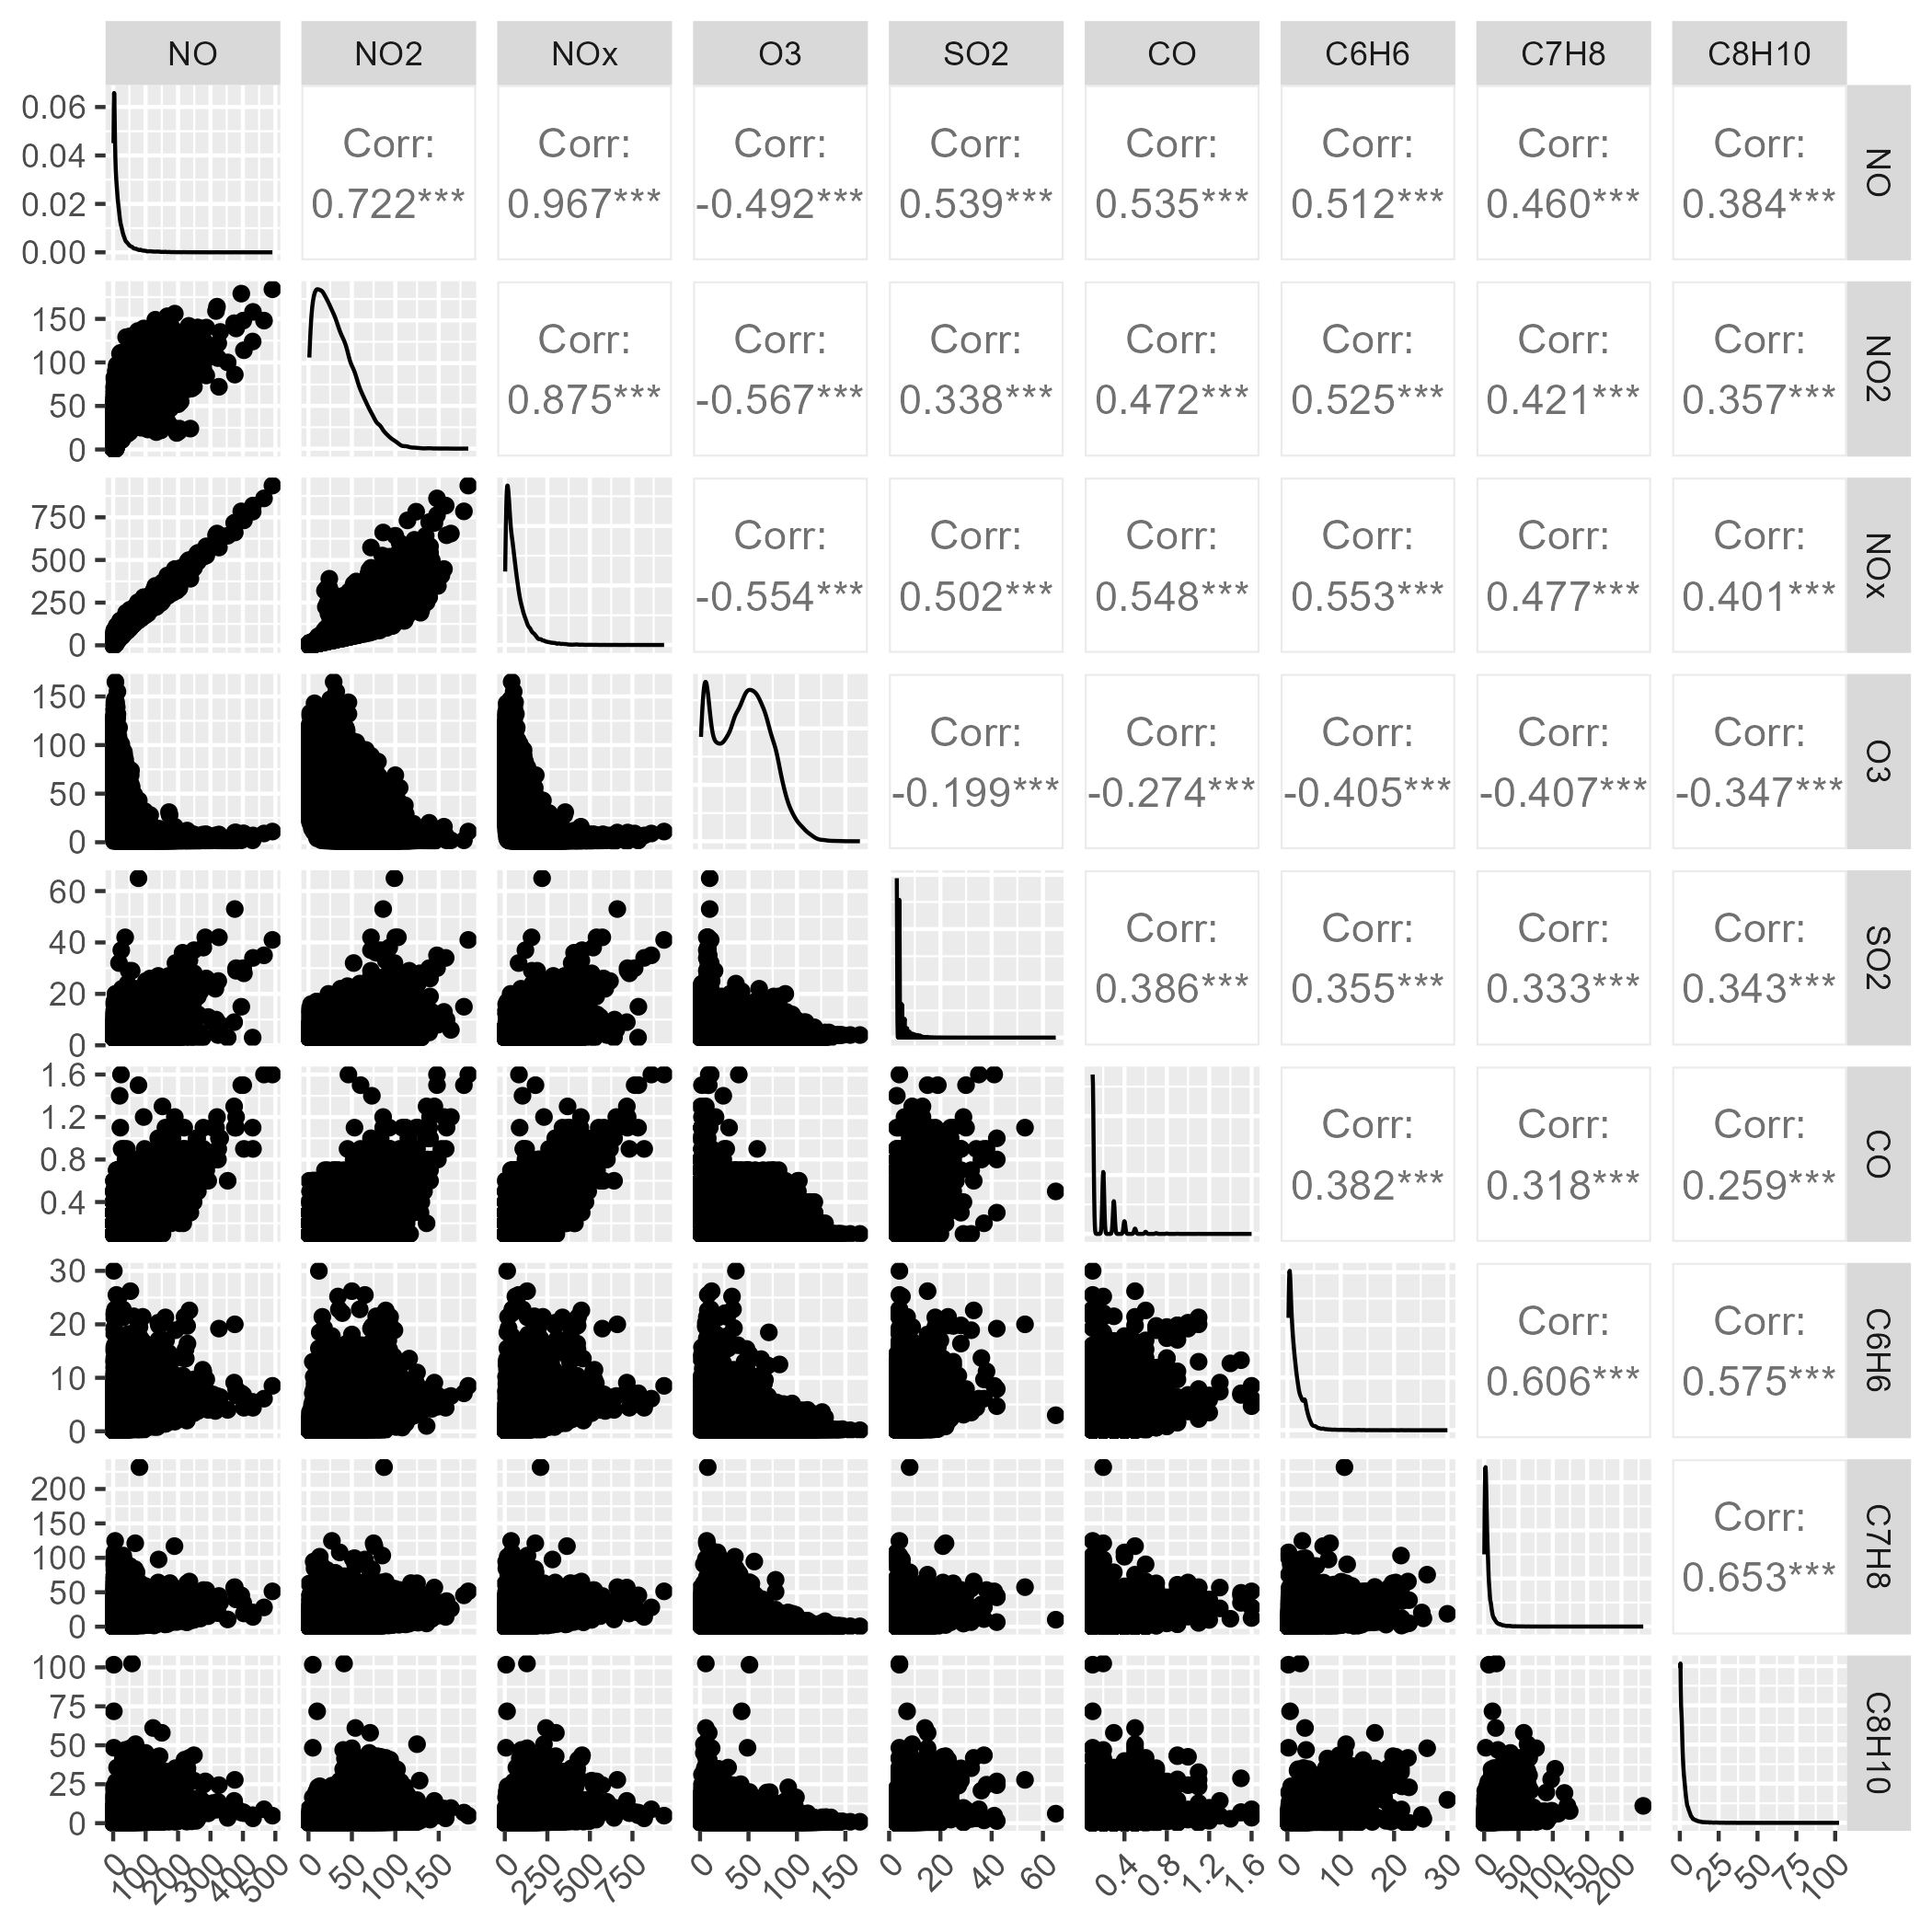
\includegraphics[width=29.17in]{grafs/correlation}

Se evidencia una relación lineal clara entre las variables NO2, NO y
NOx, con una correlación superior al 0.7 entre ellas. Esta asociación
tiene fundamentos sólidos, dado que los óxidos de nitrógeno (NOx) son
compuestos químicos formados por átomos de nitrógeno y oxígeno. Entre
los óxidos de nitrógeno más prevalentes se encuentran el óxido nítrico
(NO) y el dióxido de nitrógeno (NO2), por lo que el término NOx engloba
la mezcla de estos óxidos, indicando que un incremento en NO y NO2
conlleva un aumento en NOx.

La justificación de esta relación se encuentra en el proceso de
formación de estos compuestos, principalmente durante la combustión de
combustibles a elevadas temperaturas, como la que ocurre en motores de
vehículos, centrales eléctricas y otras instalaciones industriales. Es
relevante destacar que el NO2 es un contaminante atmosférico de
considerable importancia.

Por consiguiente, a partir de este punto, se podría considera enfocar el
análisis exclusivamente en el NOx para simplificar la investigación,
dada su representatividad y la relación intrínseca con los óxidos de
nitrógeno clave en la atmósfera.

\hypertarget{impacto-de-las-horas-de-desplazamiento-laboral-en-la-calidad-del-aire}{%
\section{Impacto de las Horas de Desplazamiento Laboral en la Calidad
del
Aire}\label{impacto-de-las-horas-de-desplazamiento-laboral-en-la-calidad-del-aire}}

Una vez hecho el análisis podemos comenzar a dar respuesta a nuestras
preguntas iniciales. Para ello, vamos a realizar la visualización de la
concentración de contaminantes por horas del día, realizando a su vez,
la comparación entre días de la semana.

\includegraphics{codigoProyecto_files/figure-latex/unnamed-chunk-19-1.pdf}
Somos capaces de apreciar los picos de contaminación en horas punta, sin
embargo, los valores de las concentraciones de hidrocarburos son bajos,
situándose en el extremo inferior de la imagen y solapándose entre
ellos. Es por ello que hemos tomado la decisión de representar estos
datos en escala logarítmica para varios días. Porque la forma de las
gráficas son muy similares en los días laborables, solo mostraremos los
martes, pero el resto de gráficas pueden consultarse en la documentación
del trabajo.

\includegraphics{codigoProyecto_files/figure-latex/unnamed-chunk-20-1.pdf}
\includegraphics{codigoProyecto_files/figure-latex/unnamed-chunk-20-2.pdf}
\includegraphics{codigoProyecto_files/figure-latex/unnamed-chunk-20-3.pdf}
\includegraphics{codigoProyecto_files/figure-latex/unnamed-chunk-20-4.pdf}

Ahora que hemos representado las concentraciones en escala logartítmica,
somos capaces percibir los picos de concentración incluso en aquellas
variables menos presentes. Es de interés estudiar la variabilidad de las
concentraciones en función del día de la semana. Porque disponemos de 9
gases para cada día de la semana para cada una de las 24h, hemos
dedicido representar los valores absolutos de concentración. Véase la
siguiente gráfica:

\includegraphics{codigoProyecto_files/figure-latex/unnamed-chunk-22-1.pdf}
Como comentábamos con anterioridad, los días lasborables y los que no
son claramente distinguibles. Las concentraciones mantienen levemente la
forma, a costa de reducir en gran medida sus valores absolutos. Esto es
debido principalmente a la ausencia de necesidad de desplazarse al
trabajo, al colegio o a otras zonas de interés.

Podemos comprobar como la conducción de vehículos emite una variedad de
gases que tienen un impacto significativo en la calidad del aire y en la
salud pública. Entre los principales contaminantes vehiculares nos
encontramos los que se registran en nuestro \texttt{dataset}. Todos
ellos son residuos típicos de los combustibles fósiles. Hemos recopilado
información sobre ellos:

\begin{itemize}
\item
  Óxidos de Nitrógeno (NO, NO\(_2\) y NO\(_x\)): Producidos durante la
  combustión a alta temperatura en motores de vehículos. Contribuyen a
  la formación de ozono troposférico y puede irritar las vías
  respiratorias.
\item
  Monóxido de Carbono (CO): Resulta de la combustión incompleta de
  carbono en el motor. Es peligroso porque interfiere con la capacidad
  de la sangre para transportar oxígeno. Puede tener efectos tóxicos.
\item
  Óxidos de Nitrógeno (NO\(_x\)): Contribuye a la formación de smog y
  afectan la calidad del aire
\item
  Hidrocarburos (C\(_6\)H\(_6\) C\(_7\)H\(_8\) y C\(_8\)H\(_10\)):
  Provienen de la evaporación de combustibles y emisiones de escape.
  Algunos hidrocarburos son cancerígenos, y otros pueden contribuir a la
  formación de ozono y smog.
\end{itemize}

El incremento sustancial de estos contaminantes durante las horas de
máximo tráfico se debe a la mayor actividad vehicular y la consiguiente
combustión de combustibles fósiles. Está muy claro que los picos de
concentración de estos gases no son casuales, ocurren en aquellos
momentos de tráfico elevado, las gráficas respaldan esta afirmación. Los
picos ocurren:

\begin{itemize}
\tightlist
\item
  En días laborables
\item
  A las horas de entrar a trabajar/estudiar.
\end{itemize}

Este fenómeno destaca la necesidad de estrategias para mitigar las
emisiones vehiculares y mejorar la calidad del aire en entornos urbanos.
Un estudio más exhaustivo podría encargarse a expertos químicos.

\hypertarget{anuxe1lisis-de-outliers}{%
\section{Análisis de outliers}\label{anuxe1lisis-de-outliers}}

A continuación, exploraremos la calidad del aire mediante boxplots que
representan las concentraciones de dos sustancias fundamentales: dióxido
de nitrógeno (NO2) y ozono (O3). Cada gráfico proporciona una visión
detallada de la distribución de estas sustancias en las distintas
estaciones de la red de vigilancia atmosférica de la ciudad de València.

\begin{Shaded}
\begin{Highlighting}[]
\NormalTok{generate\_boxplot }\OtherTok{\textless{}{-}} \ControlFlowTok{function}\NormalTok{(data, title) \{}
  \FunctionTok{boxplot}\NormalTok{(data, }\AttributeTok{main =}\NormalTok{ title,}\AttributeTok{col =} \StringTok{"lightpink"}\NormalTok{, }\AttributeTok{border =} \StringTok{"darkblue"}\NormalTok{)}
\NormalTok{\}}

\FunctionTok{par}\NormalTok{(}\AttributeTok{mfrow =} \FunctionTok{c}\NormalTok{(}\DecValTok{2}\NormalTok{, }\DecValTok{4}\NormalTok{), }\AttributeTok{mar =} \FunctionTok{c}\NormalTok{(}\DecValTok{4}\NormalTok{, }\DecValTok{4}\NormalTok{, }\DecValTok{2}\NormalTok{, }\DecValTok{1}\NormalTok{),}\AttributeTok{cex.main =} \FloatTok{0.8}\NormalTok{)}

\ControlFlowTok{for}\NormalTok{ (nombre\_df }\ControlFlowTok{in}\NormalTok{ nombres\_dataframes) \{}
\NormalTok{  df }\OtherTok{\textless{}{-}} \FunctionTok{get}\NormalTok{(nombre\_df)}
  
  \ControlFlowTok{if}\NormalTok{ (}\StringTok{"NO2"} \SpecialCharTok{\%in\%} \FunctionTok{names}\NormalTok{(df) }\SpecialCharTok{\&\&} \FunctionTok{length}\NormalTok{(df}\SpecialCharTok{$}\NormalTok{NO2) }\SpecialCharTok{\textgreater{}} \DecValTok{0}\NormalTok{) \{}
    \FunctionTok{generate\_boxplot}\NormalTok{(df}\SpecialCharTok{$}\NormalTok{NO2, }\FunctionTok{paste}\NormalTok{(}\StringTok{"Outliers NO2"}\NormalTok{, nombre\_df, }\AttributeTok{sep =} \StringTok{" "}\NormalTok{))}
\NormalTok{  \} }\ControlFlowTok{else}\NormalTok{ \{}
    \FunctionTok{cat}\NormalTok{(}\StringTok{"No se encontró la columna \textquotesingle{}NO2\textquotesingle{} en"}\NormalTok{, nombre\_df, }\StringTok{"}\SpecialCharTok{\textbackslash{}n}\StringTok{"}\NormalTok{)}
\NormalTok{  \}}
\NormalTok{\}}
\end{Highlighting}
\end{Shaded}

\begin{verbatim}
## No se encontró la columna 'NO2' en Conselleria Meteo
\end{verbatim}

\begin{figure}
\centering
\includegraphics{codigoProyecto_files/figure-latex/fig3-1.pdf}
\caption{Diagramas de caja de NO2 en cada estación.\label{fig:fig3}}
\end{figure}

\begin{verbatim}
## No se encontró la columna 'NO2' en Nazaret Meteo
\end{verbatim}

Observamos una notable presencia de outliers en la variable \texttt{NO2}
en todas las estaciones, destacando en la parte superior de los
boxplots. Estos boxplots son estrechos, lo que sugiere que la mayor
parte de los datos se concentra en un rango reducido de concentraciones
de dióxido de nitrógeno. Sin embargo, la presencia de numerosos outliers
en la parte superior indica que a menudo se generan concentraciones
inusualmente altas de esta sustancia en el aire.

\begin{Shaded}
\begin{Highlighting}[]
\FunctionTok{par}\NormalTok{(}\AttributeTok{mfrow =} \FunctionTok{c}\NormalTok{(}\DecValTok{2}\NormalTok{, }\DecValTok{4}\NormalTok{), }\AttributeTok{mar =} \FunctionTok{c}\NormalTok{(}\DecValTok{4}\NormalTok{, }\DecValTok{4}\NormalTok{, }\DecValTok{2}\NormalTok{, }\DecValTok{1}\NormalTok{),}\AttributeTok{cex.main =} \FloatTok{0.8}\NormalTok{)}

\ControlFlowTok{for}\NormalTok{ (nombre\_df }\ControlFlowTok{in}\NormalTok{ nombres\_dataframes) \{}
\NormalTok{  df }\OtherTok{\textless{}{-}} \FunctionTok{get}\NormalTok{(nombre\_df)}
  
  \ControlFlowTok{if}\NormalTok{ (}\StringTok{"O3"} \SpecialCharTok{\%in\%} \FunctionTok{names}\NormalTok{(df) }\SpecialCharTok{\&\&} \FunctionTok{length}\NormalTok{(df}\SpecialCharTok{$}\NormalTok{O3) }\SpecialCharTok{\textgreater{}} \DecValTok{0}\NormalTok{) \{}
    \FunctionTok{generate\_boxplot}\NormalTok{(df}\SpecialCharTok{$}\NormalTok{O3, }\FunctionTok{paste}\NormalTok{(}\StringTok{"Outliers O3"}\NormalTok{, nombre\_df, }\AttributeTok{sep =} \StringTok{" "}\NormalTok{))}
\NormalTok{  \} }\ControlFlowTok{else}\NormalTok{ \{}
    \FunctionTok{cat}\NormalTok{(}\StringTok{"No se encontró la columna \textquotesingle{}O3\textquotesingle{} en"}\NormalTok{, nombre\_df, }\StringTok{"}\SpecialCharTok{\textbackslash{}n}\StringTok{"}\NormalTok{)}
\NormalTok{  \}}
\NormalTok{\}}
\end{Highlighting}
\end{Shaded}

\begin{verbatim}
## No se encontró la columna 'O3' en Conselleria Meteo
\end{verbatim}

\begin{verbatim}
## No se encontró la columna 'O3' en Valencia Centro 
## No se encontró la columna 'O3' en Nazaret Meteo
\end{verbatim}

\includegraphics{codigoProyecto_files/figure-latex/fig4-1.pdf} En
contraste, la presencia de outliers en la variable de ozono es menos
pronunciada. Aunque en las estaciones de Viveros y Consellería Meteo se
observa una mayor proporción de outliers, en general, los valores
presentan una distribución más uniforme. Los boxplots son más anchos,
indicando una dispersión más amplia de las concentraciones de ozono.

También hemos considerado oportuno implementar funciones específicas
para la identificación de outliers utilizando distintos métodos
estadísticos, como la regla de 3 sigma, el identificador Hampel y la
regla de percentiles. Este es otro modo de resaltar valores que podrían
considerarse atípicos y podemos comparar con los resultados obtenidos
mediante el método boxplot.

Función para la regla de 3 sigma:

\begin{Shaded}
\begin{Highlighting}[]
\NormalTok{reglasigma }\OtherTok{\textless{}{-}} \ControlFlowTok{function}\NormalTok{(x) \{}
\NormalTok{  media }\OtherTok{\textless{}{-}} \FunctionTok{mean}\NormalTok{(x, }\AttributeTok{na.rm =} \ConstantTok{TRUE}\NormalTok{)}
\NormalTok{  desviacion }\OtherTok{\textless{}{-}} \FunctionTok{sd}\NormalTok{(x, }\AttributeTok{na.rm =} \ConstantTok{TRUE}\NormalTok{)}
\NormalTok{  umbral\_superior }\OtherTok{\textless{}{-}}\NormalTok{ media }\SpecialCharTok{+} \DecValTok{3} \SpecialCharTok{*}\NormalTok{ desviacion}
\NormalTok{  umbral\_inferior }\OtherTok{\textless{}{-}}\NormalTok{ media }\SpecialCharTok{{-}} \DecValTok{3} \SpecialCharTok{*}\NormalTok{ desviacion}
\NormalTok{  outliers }\OtherTok{\textless{}{-}}\NormalTok{ x[x }\SpecialCharTok{\textgreater{}}\NormalTok{ umbral\_superior }\SpecialCharTok{|}\NormalTok{ x }\SpecialCharTok{\textless{}}\NormalTok{ umbral\_inferior]}
  \FunctionTok{return}\NormalTok{(outliers)}
\NormalTok{\}}
\end{Highlighting}
\end{Shaded}

Función para el identificador Hampel:

\begin{Shaded}
\begin{Highlighting}[]
\NormalTok{reglahampel }\OtherTok{\textless{}{-}} \ControlFlowTok{function}\NormalTok{(x) \{}
\NormalTok{  mediana }\OtherTok{\textless{}{-}} \FunctionTok{median}\NormalTok{(x, }\AttributeTok{na.rm =} \ConstantTok{TRUE}\NormalTok{)}
\NormalTok{  mad }\OtherTok{\textless{}{-}} \FunctionTok{mad}\NormalTok{(x, }\AttributeTok{na.rm =} \ConstantTok{TRUE}\NormalTok{)}
\NormalTok{  umbral\_superior }\OtherTok{\textless{}{-}}\NormalTok{ mediana }\SpecialCharTok{+} \DecValTok{3} \SpecialCharTok{*}\NormalTok{ mad}
\NormalTok{  umbral\_inferior }\OtherTok{\textless{}{-}}\NormalTok{ mediana }\SpecialCharTok{{-}} \DecValTok{3} \SpecialCharTok{*}\NormalTok{ mad}
\NormalTok{  outliers }\OtherTok{\textless{}{-}}\NormalTok{ x[x }\SpecialCharTok{\textgreater{}}\NormalTok{ umbral\_superior }\SpecialCharTok{|}\NormalTok{ x }\SpecialCharTok{\textless{}}\NormalTok{ umbral\_inferior]}
  \FunctionTok{return}\NormalTok{(outliers)}
\NormalTok{\}}
\end{Highlighting}
\end{Shaded}

Función para la regla del boxplot:

\begin{Shaded}
\begin{Highlighting}[]
\NormalTok{reglaboxplot }\OtherTok{\textless{}{-}} \ControlFlowTok{function}\NormalTok{(x) \{}
\NormalTok{  cuartil\_75 }\OtherTok{\textless{}{-}} \FunctionTok{quantile}\NormalTok{(x, }\FloatTok{0.75}\NormalTok{, }\AttributeTok{na.rm =} \ConstantTok{TRUE}\NormalTok{)}
\NormalTok{  cuartil\_25 }\OtherTok{\textless{}{-}} \FunctionTok{quantile}\NormalTok{(x, }\FloatTok{0.25}\NormalTok{, }\AttributeTok{na.rm =} \ConstantTok{TRUE}\NormalTok{)}
\NormalTok{  iqr }\OtherTok{\textless{}{-}}\NormalTok{ cuartil\_75 }\SpecialCharTok{{-}}\NormalTok{ cuartil\_25}
\NormalTok{  umbral\_superior }\OtherTok{\textless{}{-}}\NormalTok{ cuartil\_75 }\SpecialCharTok{+} \FloatTok{1.5} \SpecialCharTok{*}\NormalTok{ iqr}
\NormalTok{  umbral\_inferior }\OtherTok{\textless{}{-}}\NormalTok{ cuartil\_25 }\SpecialCharTok{{-}} \FloatTok{1.5} \SpecialCharTok{*}\NormalTok{ iqr}
\NormalTok{  outliers }\OtherTok{\textless{}{-}}\NormalTok{ x[x }\SpecialCharTok{\textgreater{}}\NormalTok{ umbral\_superior }\SpecialCharTok{|}\NormalTok{ x }\SpecialCharTok{\textless{}}\NormalTok{ umbral\_inferior]}
  \FunctionTok{return}\NormalTok{(outliers)}
\NormalTok{\}}
\end{Highlighting}
\end{Shaded}

Función para la regla de percentiles:

\begin{Shaded}
\begin{Highlighting}[]
\NormalTok{reglapercentil }\OtherTok{\textless{}{-}} \ControlFlowTok{function}\NormalTok{(x) \{}
\NormalTok{  percentil\_5 }\OtherTok{\textless{}{-}} \FunctionTok{quantile}\NormalTok{(x, }\FloatTok{0.05}\NormalTok{, }\AttributeTok{na.rm =} \ConstantTok{TRUE}\NormalTok{)}
\NormalTok{  percentil\_95 }\OtherTok{\textless{}{-}} \FunctionTok{quantile}\NormalTok{(x, }\FloatTok{0.95}\NormalTok{, }\AttributeTok{na.rm =} \ConstantTok{TRUE}\NormalTok{)}
\NormalTok{  outliers }\OtherTok{\textless{}{-}}\NormalTok{ x[x }\SpecialCharTok{\textless{}}\NormalTok{ percentil\_5 }\SpecialCharTok{|}\NormalTok{ x }\SpecialCharTok{\textgreater{}}\NormalTok{ percentil\_95]}
  \FunctionTok{return}\NormalTok{(outliers)}
\NormalTok{\}}
\end{Highlighting}
\end{Shaded}

\begin{Shaded}
\begin{Highlighting}[]
\NormalTok{detectar\_outliers }\OtherTok{\textless{}{-}} \ControlFlowTok{function}\NormalTok{(x) \{}
\NormalTok{  sol }\OtherTok{\textless{}{-}} \FunctionTok{list}\NormalTok{(}
    \AttributeTok{r\_sigma =} \FunctionTok{data.frame}\NormalTok{(}\AttributeTok{Variable =} \FunctionTok{colnames}\NormalTok{(x), }\AttributeTok{Metodo =} \StringTok{"Regla 3 sigma"}\NormalTok{, }
              \AttributeTok{Outliers =} \FunctionTok{sapply}\NormalTok{(x, }\ControlFlowTok{function}\NormalTok{(col) }\FunctionTok{length}\NormalTok{(}\FunctionTok{reglasigma}\NormalTok{(col)))),}
    \AttributeTok{r\_hampel =} \FunctionTok{data.frame}\NormalTok{(}\AttributeTok{Variable =} \FunctionTok{colnames}\NormalTok{(x), }\AttributeTok{Metodo =} \StringTok{"Identificador Hampel"}\NormalTok{, }
               \AttributeTok{Outliers =} \FunctionTok{sapply}\NormalTok{(x, }\ControlFlowTok{function}\NormalTok{(col) }\FunctionTok{length}\NormalTok{(}\FunctionTok{reglahampel}\NormalTok{(col)))),}
    \AttributeTok{r\_boxplot =} \FunctionTok{data.frame}\NormalTok{(}\AttributeTok{Variable =} \FunctionTok{colnames}\NormalTok{(x), }\AttributeTok{Metodo =} \StringTok{"Regla Boxplot"}\NormalTok{, }
                \AttributeTok{Outliers =} \FunctionTok{sapply}\NormalTok{(x, }\ControlFlowTok{function}\NormalTok{(col) }\FunctionTok{length}\NormalTok{(}\FunctionTok{reglaboxplot}\NormalTok{(col)))),}
    \AttributeTok{r\_percentiles =} \FunctionTok{data.frame}\NormalTok{(}\AttributeTok{Variable =} \FunctionTok{colnames}\NormalTok{(x), }\AttributeTok{Metodo =} \StringTok{"Regla Percentiles"}\NormalTok{, }
                    \AttributeTok{Outliers =} \FunctionTok{sapply}\NormalTok{(x, }\ControlFlowTok{function}\NormalTok{(col) }\FunctionTok{length}\NormalTok{(}\FunctionTok{reglapercentil}\NormalTok{(col))))}
\NormalTok{  )}

  \FunctionTok{return}\NormalTok{(sol)}
\NormalTok{\}}


\NormalTok{columnas\_a\_excluir }\OtherTok{\textless{}{-}} \FunctionTok{c}\NormalTok{(}\DecValTok{1}\SpecialCharTok{:}\DecValTok{6}\NormalTok{, }\FunctionTok{ncol}\NormalTok{(df))}
\NormalTok{col }\OtherTok{\textless{}{-}} \FunctionTok{setdiff}\NormalTok{(}\FunctionTok{names}\NormalTok{(df), }\FunctionTok{names}\NormalTok{(df)[columnas\_a\_excluir])}
\NormalTok{outliers\_resultados }\OtherTok{\textless{}{-}} \FunctionTok{detectar\_outliers}\NormalTok{(Viveros[col])}

\NormalTok{plots }\OtherTok{\textless{}{-}} \FunctionTok{lapply}\NormalTok{(outliers\_resultados, }\ControlFlowTok{function}\NormalTok{(result) \{}
  \FunctionTok{ggplot}\NormalTok{(result, }\FunctionTok{aes}\NormalTok{(}\AttributeTok{x =}\NormalTok{ Variable, }\AttributeTok{y =}\NormalTok{ Outliers, }\AttributeTok{fill =}\NormalTok{ Variable)) }\SpecialCharTok{+}
    \FunctionTok{geom\_bar}\NormalTok{(}\AttributeTok{stat =} \StringTok{"identity"}\NormalTok{) }\SpecialCharTok{+}
    \FunctionTok{labs}\NormalTok{(}\AttributeTok{title =} \FunctionTok{unique}\NormalTok{(result}\SpecialCharTok{$}\NormalTok{Metodo),}
         \AttributeTok{x =} \StringTok{"Variable"}\NormalTok{,}
         \AttributeTok{y =} \StringTok{"Cantidad de Outliers"}\NormalTok{) }\SpecialCharTok{+}
    \FunctionTok{theme\_minimal}\NormalTok{() }\SpecialCharTok{+} \FunctionTok{theme}\NormalTok{(}\AttributeTok{axis.text.x =} \FunctionTok{element\_blank}\NormalTok{(), }\AttributeTok{legend.position =} \StringTok{"none"}\NormalTok{)}
\NormalTok{\})}

\FunctionTok{grid.arrange}\NormalTok{(}\AttributeTok{grobs =}\NormalTok{ plots, }\AttributeTok{ncol =} \DecValTok{2}\NormalTok{)}
\end{Highlighting}
\end{Shaded}

\begin{figure}
\centering
\includegraphics{codigoProyecto_files/figure-latex/fig5-1.pdf}
\caption{Gráficos de barras para detectar outliers.\label{fig:fig5}}
\end{figure}

La información resultante se presenta de manera clara y comparativa a
través de gráficos de barras. Cada barra en estos gráficos representa la
cantidad de outliers detectados para una variable específica, empleando
diferentes métodos de detección. En este caso, lo hemos aplicado sobre
los datos de la estación Viveros.

\hypertarget{conclusiones}{%
\section{Conclusiones}\label{conclusiones}}

\end{document}
